\subsection{Equilibrium results}
\label{subsec:monte_carlo_results}
First we look into relation between order parameter~\eqref{eq:nematic_order_parameter} and $k_BT$ at equilibrium for different system densities. As we can see on the Figure~\ref{fig:op_kbt}, the nematic order increases with decrease of $k_BT$. Important to observer rapid increase in order parameter. The region of rapid increase shifts with densities, and for high density the relation between order parameter and $k_BT$ approaches linear. Black color shows results for $N = 1600$ and red color for $N = 3200$ particles. As we can see there is no systematic scaling with system size. The results are average over $500$ samples.

\begin{figure}[h]
	\centering
	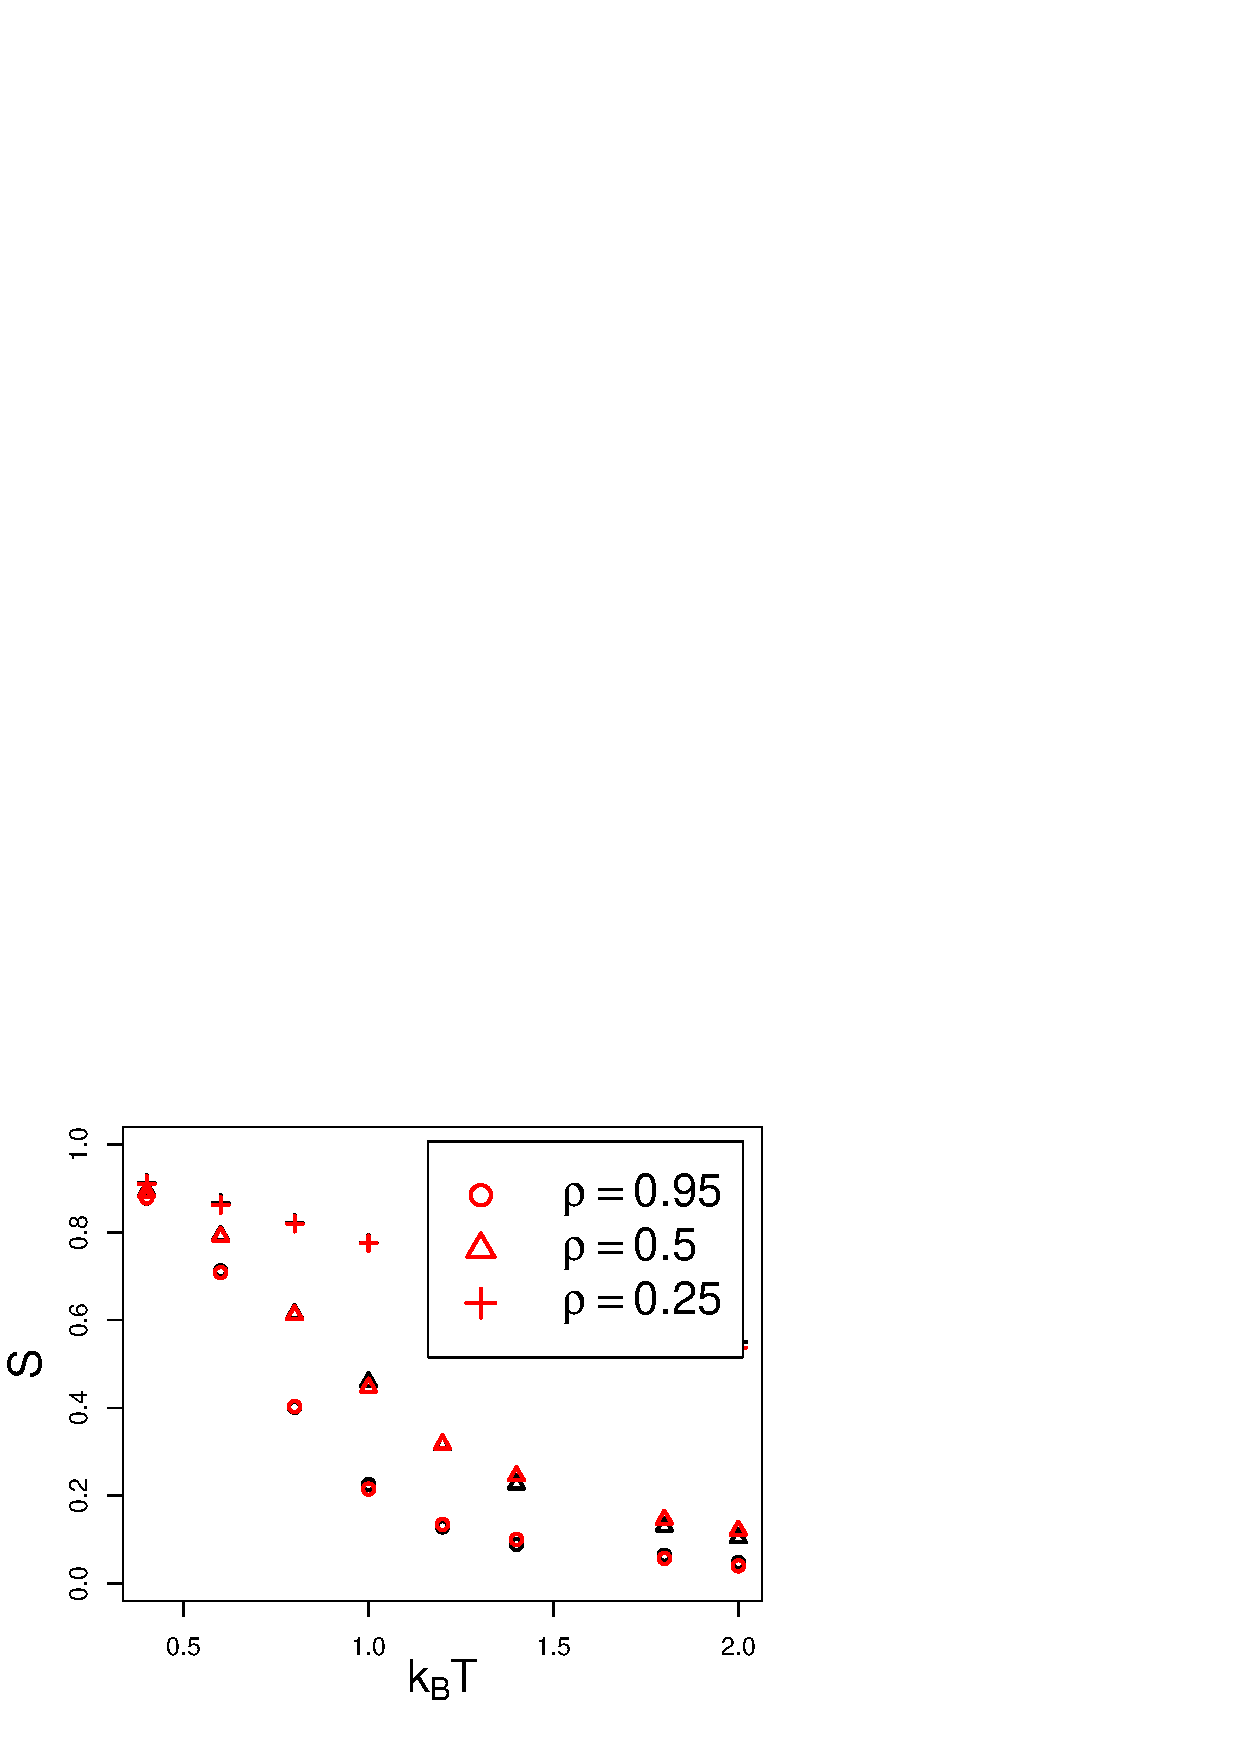
\includegraphics[width=0.5\textwidth]{Images/op_vs_kbt_MC.png}
	\captionsetup{justification=centering, width=0.9\columnwidth}
	\caption{Order parameter defined by eq.~\eqref{eq:nematic_order_parameter} versus $k_BT$ for Monte-Carlo simulations. RED shows results for $N = 3200$, and BLACK shows results for $N = 1600$. The results are average over $500$ samples \textcolor{red}{replace} as described in sec.~\ref{subsec:simulation_details}}
	\label{fig:op_kbt}
\end{figure}

Growth of order parameter with decrease of temperature may imply structural changes in observed system. To investigate that, we first calculate the probability of having two chains pointing in the same direction (along or counter $z$ axis) or in opposite directions for different $k_BT$.

Next we look into orientation correlation at equilibrium. On the \figref{fig:correlation_equilibrium} we can see that for all values of $k_BT$ the correlations decay exponentially. The factor of the exponent grows with density, as shown on sub-figures. The simulations were done for $N = 1600$ particles, and the results are averaged over $200$ samples.

\begin{figure}[p]
	\centering
	\begin{subfigure}{\textwidth}
	\centering
		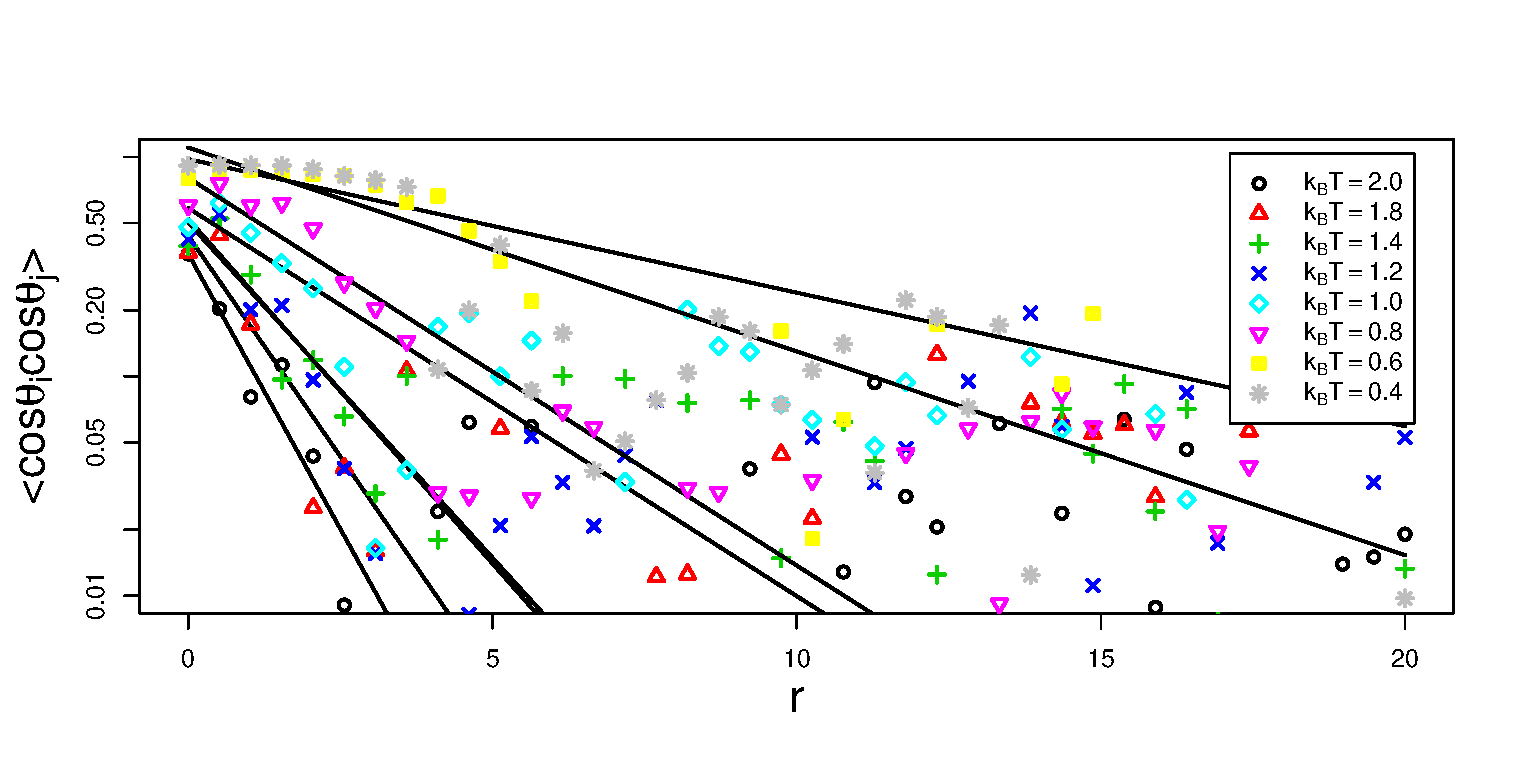
\includegraphics[height = 5cm]{Images/correlations_025}
		\captionsetup{justification=centering, width=0.9\columnwidth}
		\caption{$\rho = 0.25$}
	\end{subfigure}
	\begin{subfigure}{\textwidth}
	\centering
		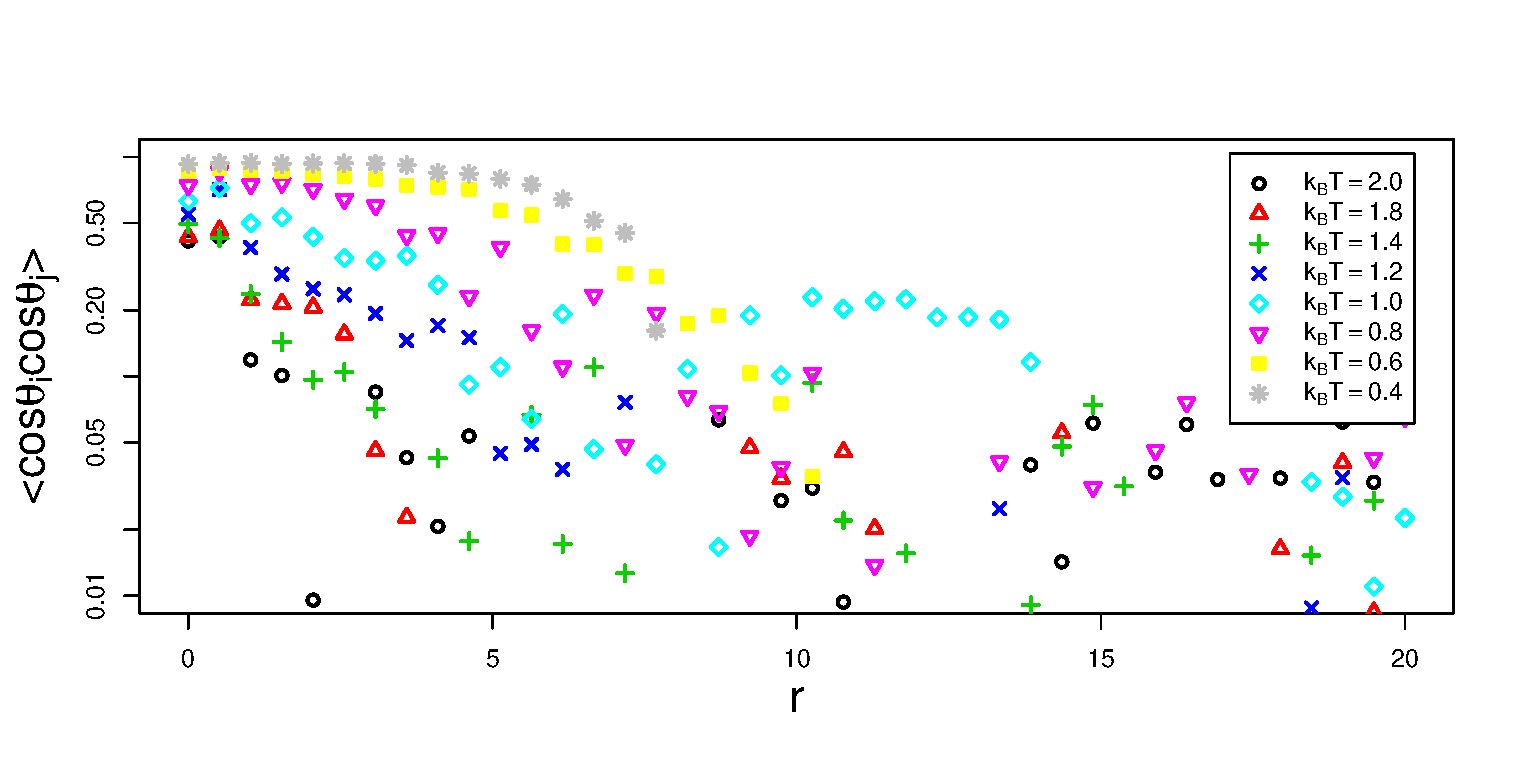
\includegraphics[height = 5cm]{Images/correlations_05}
		\captionsetup{justification=centering, width=0.9\columnwidth}
		\caption{$\rho = 0.5$}
	\end{subfigure}
	\begin{subfigure}{\textwidth}
	\centering
		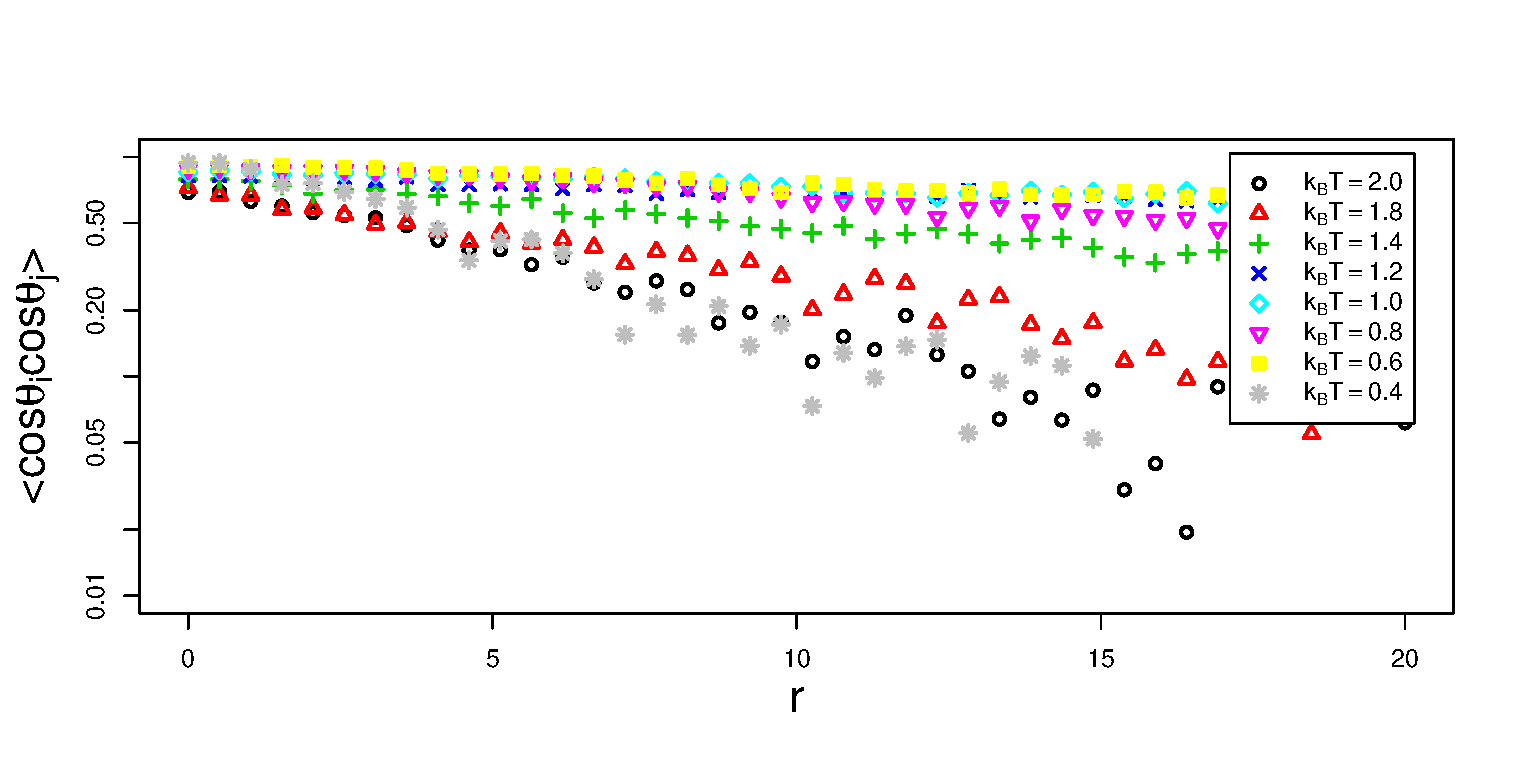
\includegraphics[height = 5cm]{Images/correlations_095}
		\captionsetup{justification=centering, width=0.9\columnwidth}
		\caption{$\rho = 0.95$}
	\end{subfigure}
	\captionsetup{justification=centering, width=0.9\columnwidth}
	\caption{Equilibrium orientation correlation as function of distance for different values of density $\rho$ and $k_BT$. Points are results of simulations done for $N = 1600$ particles, and averaged over $200$ samples. Solid lines are exponential approximation of results below certain cut-off distance. \textcolor{red}{I mean, that's fitting of the exponent by first points, but the cut-off is different for different density}}
	\label{fig:correlation_equilibrium}
\end{figure}

If we look how the slope of the correlation length depends on the $k_BT$ (\figref{fig:correlation_slopes}, we find that it, first, decays linearly with temperature, and second, for low density slope of decay does not depend on the value of density. \textcolor{red}{I take the exponent line which is shown on the \ref{fig:correlation_equilibrium}. Should I elaborate on that or it's obvious?}

\begin{figure}[t]
	\centering
	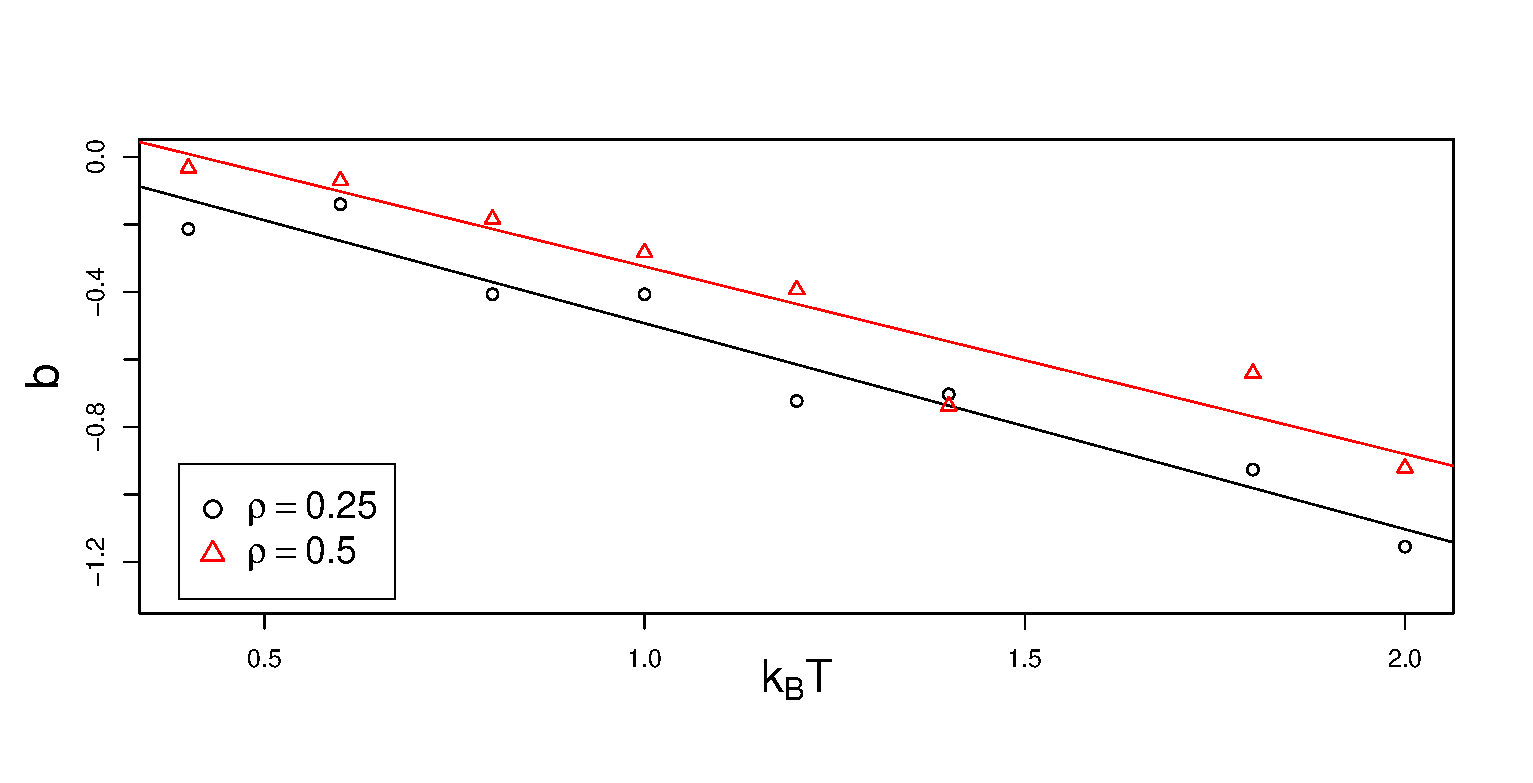
\includegraphics[width=.7\textwidth]{Images/correlations_slopes}
	\captionsetup{justification=centering, width=0.9\columnwidth}
	\caption{Slopes of orientation correlation as function of $k_BT$ for different densities. Points are obtained fitting exponential function to results of Monte-Carlo simulations presented on \figref{fig:correlation_equilibrium}  and solid lines are linear approximations}
	\label{fig:correlation_slopes}
\end{figure}